\documentclass{article}
\usepackage[utf8]{inputenc}
\usepackage[letterpaper, portrait, margin=0.2in]{geometry}
\usepackage{multicol}
\usepackage{amsmath}
\usepackage{amssymb}
\usepackage{enumerate}
\setlength\parindent{0pt}
\usepackage{enumerate}
\usepackage{graphicx}
\graphicspath{ {../images/} }
\usepackage{fancyhdr}
\usepackage{tcolorbox}
\usepackage[fontsize=8pt]{fontsize}
\usepackage[none]{hyphenat}
\usepackage[document]{ragged2e}

\newcommand{\sepvec}{\vec{r_\textrm{sep}}}
\newcommand{\sephat}{\hat{r}_{\textrm{sep}}}
\newcommand{\kfrac}{\frac{1}{4\pi\epsilon_0}}

\newcommand{\header}[1]{\begin{large}\noindent #1\end{large}\\\rule{\textwidth}{0.5pt}}
\newcommand{\gap}{\medskip\\}
\newcommand{\centertext}[1]{\begin{center}#1\end{center}}
\newcommand{\bfrac}[2]{\left(\frac{#1}{#2}\right)}
\newcommand{\formula}[2]{\begin{center} \begin{tcolorbox}[title = #1, boxrule=2pt,arc=3.4pt,boxsep=0mm] $$#2$$\end{tcolorbox}\end{center}}
\newcommand{\doubleformula}[3]{\begin{center} \begin{tcolorbox}[title = #1, boxrule=2pt,arc=3.4pt,boxsep=0mm] $$#2$$\\$$#3$$\end{tcolorbox}\end{center}}
\newcommand{\formulax}[2]{\underline{#1}\smallskip\centering $#2$ \raggedleft}
\newcommand{\tripleformula}[5]{\begin{center} \begin{tcolorbox}[title = #2, boxrule=2pt,arc=3.4pt,boxsep=0mm] $$#3$$\\$$#4$$\\$$#5$$\end{tcolorbox}\end{center}}

\newcommand{\formbox}[2]{\begin{center} \begin{tcolorbox}[title = #1, boxrule=2pt,arc=3.4pt,boxsep=0mm] #2\end{tcolorbox}\end{center}}


\newcommand{\where}{\hspace{0.3cm} \textrm{where} \hspace{0.3cm}}



\begin{document}

\begin{multicols*}{3}

\doubleformula{Taylor Expansion}{f(x) \approx \sum_{n=0}^\infty \frac{f^{(n)}(0)}{n!}}{f(x) \approx f(0) + f'(0) \cdot x + f''(0) \cdot \frac{x^2}{2} + \cdots}
\formbox{Field Integrals}{
\centertext{Line Charge}
\[\vec{E}(\vec{r}) = \frac{1}{4 \pi \epsilon_0}\int{\frac{\lambda(\vec{r'})}{||\sepvec||^2}\sephat \, dl'}\]
\centertext{Surface Charge}
\[\vec{E}(\vec{r}) = \frac{1}{4\pi\epsilon_0}\int{\frac{\sigma(\vec{r'})}{||\sepvec||^2}\sephat \, da'}\]
\centertext{Volume Charge}
\[\vec{E}(\vec{r}) = \frac{1}{4\pi\epsilon_0}\int{\frac{\rho(\vec{r'})}{||\sepvec||^2}\sephat \, d\tau'}\]
}

\formula{Potential Difference}{V(\vec{b}) - V(\vec{a}) = - \int_{\vec{a}}^{\vec{b}}{\vec{E} \cdot d\vec{l}}}

\formbox{Potentials}{
\centertext{Volume Charge}
\[V(\vec{r}) = \kfrac \int{\frac{\rho(\vec{r'})}{||\sepvec||}d\tau'}\]
\centertext{Collection of Point Charges}
\[V(\vec{r}) = \kfrac \sum_{i = 0}^n\frac{q_i}{||\sepvec||}\]
}

\doubleformula{Work to Move a Charge}{W = \int_{\textbf{a}}^{\textbf{b}} \vec{F} \cdot d\vec{l} = -Q\int_{\textbf{a}}^{\textbf{b}}{\vec{E} \cdot d\vec{l}}}{W= Q[V(\vec{b}) - Q(\vec{a})]}

\formbox{Energy of a Charge Distributions}{
\centertext{Collection of Point Charges}
\[W = \frac{1}{2}\sum_{i = 1}^n{q_i V(\vec{r_i})}\]
\centertext{Continuous Charge Distribution}
\[W = \frac{\epsilon_0}{2}\int\limits_{\textrm{all space}}E^2 d\tau\]
}
\begin{multicols*}{2}

\formula{Parallel Plate Voltage}{V = \frac{Q}{A\epsilon_0}d}
\vfill\null\columnbreak
\formula{Capacitance}{C \equiv \frac{Q}{V}}
\vfill\null
\end{multicols*}


\formula{Energy of a Capacitor}{
    W = \int_0^Q{\bfrac{q}{C}dq} = \frac{1}{2}\frac{Q^2}{C} = \frac{1}{2} CV^2
}

\formbox{Common Boundary Conditions}{
\centertext{\underline{Continuity of Potential}}
\[
    V_\textrm{above}(a) = V_\textrm{below}(a)
\]
\centertext{\underline{Preservation of Field}\\
(Symmetry Required)}
\[
    \vec{E}_\textrm{above} - \vec{E}_\textrm{below} = \frac{\sigma}{\epsilon_0}\hat{n}
\]
\centertext{\underline{Bounding of Origin}\\
(Generally Spherical Distributions)}
\[
    V(0) \textrm{ is bounded.}        
\]
\centertext{\underline{Bounding of Infinity}\\
(Generally Spherical Distributions)}
\[
    V(\infty) = 0.    
\]
}

\formbox{Uniqueness of Solutions}{
    For a charge distribution with $\nabla^2V = 0$:
    \begin{enumerate}
        \item $V$ has no local maxima nor minima inside. The maxima and minima are located
        on the surrounding boundaries.
        \item $V$ is smooth and continuous, everywhere.
        \item $V(\vec{r})$ is the average of $V$ over surface of any surrounding sphere:
        $V(\vec{r}) = \frac{1}{4\pi R^2}\oint VdA$.
        \item $V$ is unique, as the solution of the Laplace equation is uniquely determined
        if $V$ is specified on the boundary surface around the volume.
    \end{enumerate}
}

\formbox{Earnshaw's Theorem}{
A charged particle cannot be held in a stable equilibrium by electrostatic forces alone.
This can be analyzed using divergence amongst other methods of analysis.
}

\formbox{Properties of Conductors}{
    \begin{enumerate}
        \item \underline{$\vec{E} = 0$ inside a conductor}. In short, charges move to oppose any external $\vec{E}$ fields.
        This can also be interpreted under the principle that if there was any field inside
        a conductor, the free electrons would be moving, and hence not \textit{electrostatic}.
        \item Any net charges reside on the surface of a conductor.
        \item \underline{$\rho = 0$ inside a conductor}. Since there is no field inside a conductor,
        Gauss's law requires that there is no enclosed charge, thus, there is no charge density.
        One may make the argument for the surface charges, however, since they are equal in magnitude,
        they cancel.
        \item \underline{A conductor is an equipotential}. Since there is no field inside
        a conductor, given the relationship $\nabla V = -\vec{E}$, the potential $V$ must
        be a constant.
        \item $\vec{E}$ is $\perp$ to the surface of a conductor.
    \end{enumerate} 
}

\formbox{Rules for Irrotational Fields}{
    Since all electrostatic fields are conservative and therefore irrotational:
    \begin{enumerate}
        \item $\vec{\nabla} \times \vec{F} = \vec{0}$ everywhere.
        \item $\int_a^b\vec{F}\cdot d\vec{l}$ is independent of path, for any given end points.
        \item $\oint \vec{F}\cdot d\vec{l} = 0$ for any closed loop.
        \item $\vec{F}$ is the gradient of some scalar function: $\vec{F} = -\nabla V$.
    \end{enumerate}
}

\formbox{Problem Solving Stragegy -- Coulomb Integrals}{
    \begin{enumerate}
        \item Choose a coordinate system.
        \item Identify $\vec{r}$, the vector from the origin to the point of interest.
        \item Identify $\vec{r'}$, the vector from the origin to the charge distribution.
        \item Identify $\sepvec$, the vector separating the charge distribution and the point of interest:
        $(\sepvec = \vec{r} - \vec{r'})$
        \item If possible, identify any symmetries to try to solve the problem with.
        \item Integrate.
    \end{enumerate}
}

\formbox{The Electricity and Magnetism Triangle}{
    \begin{center}
        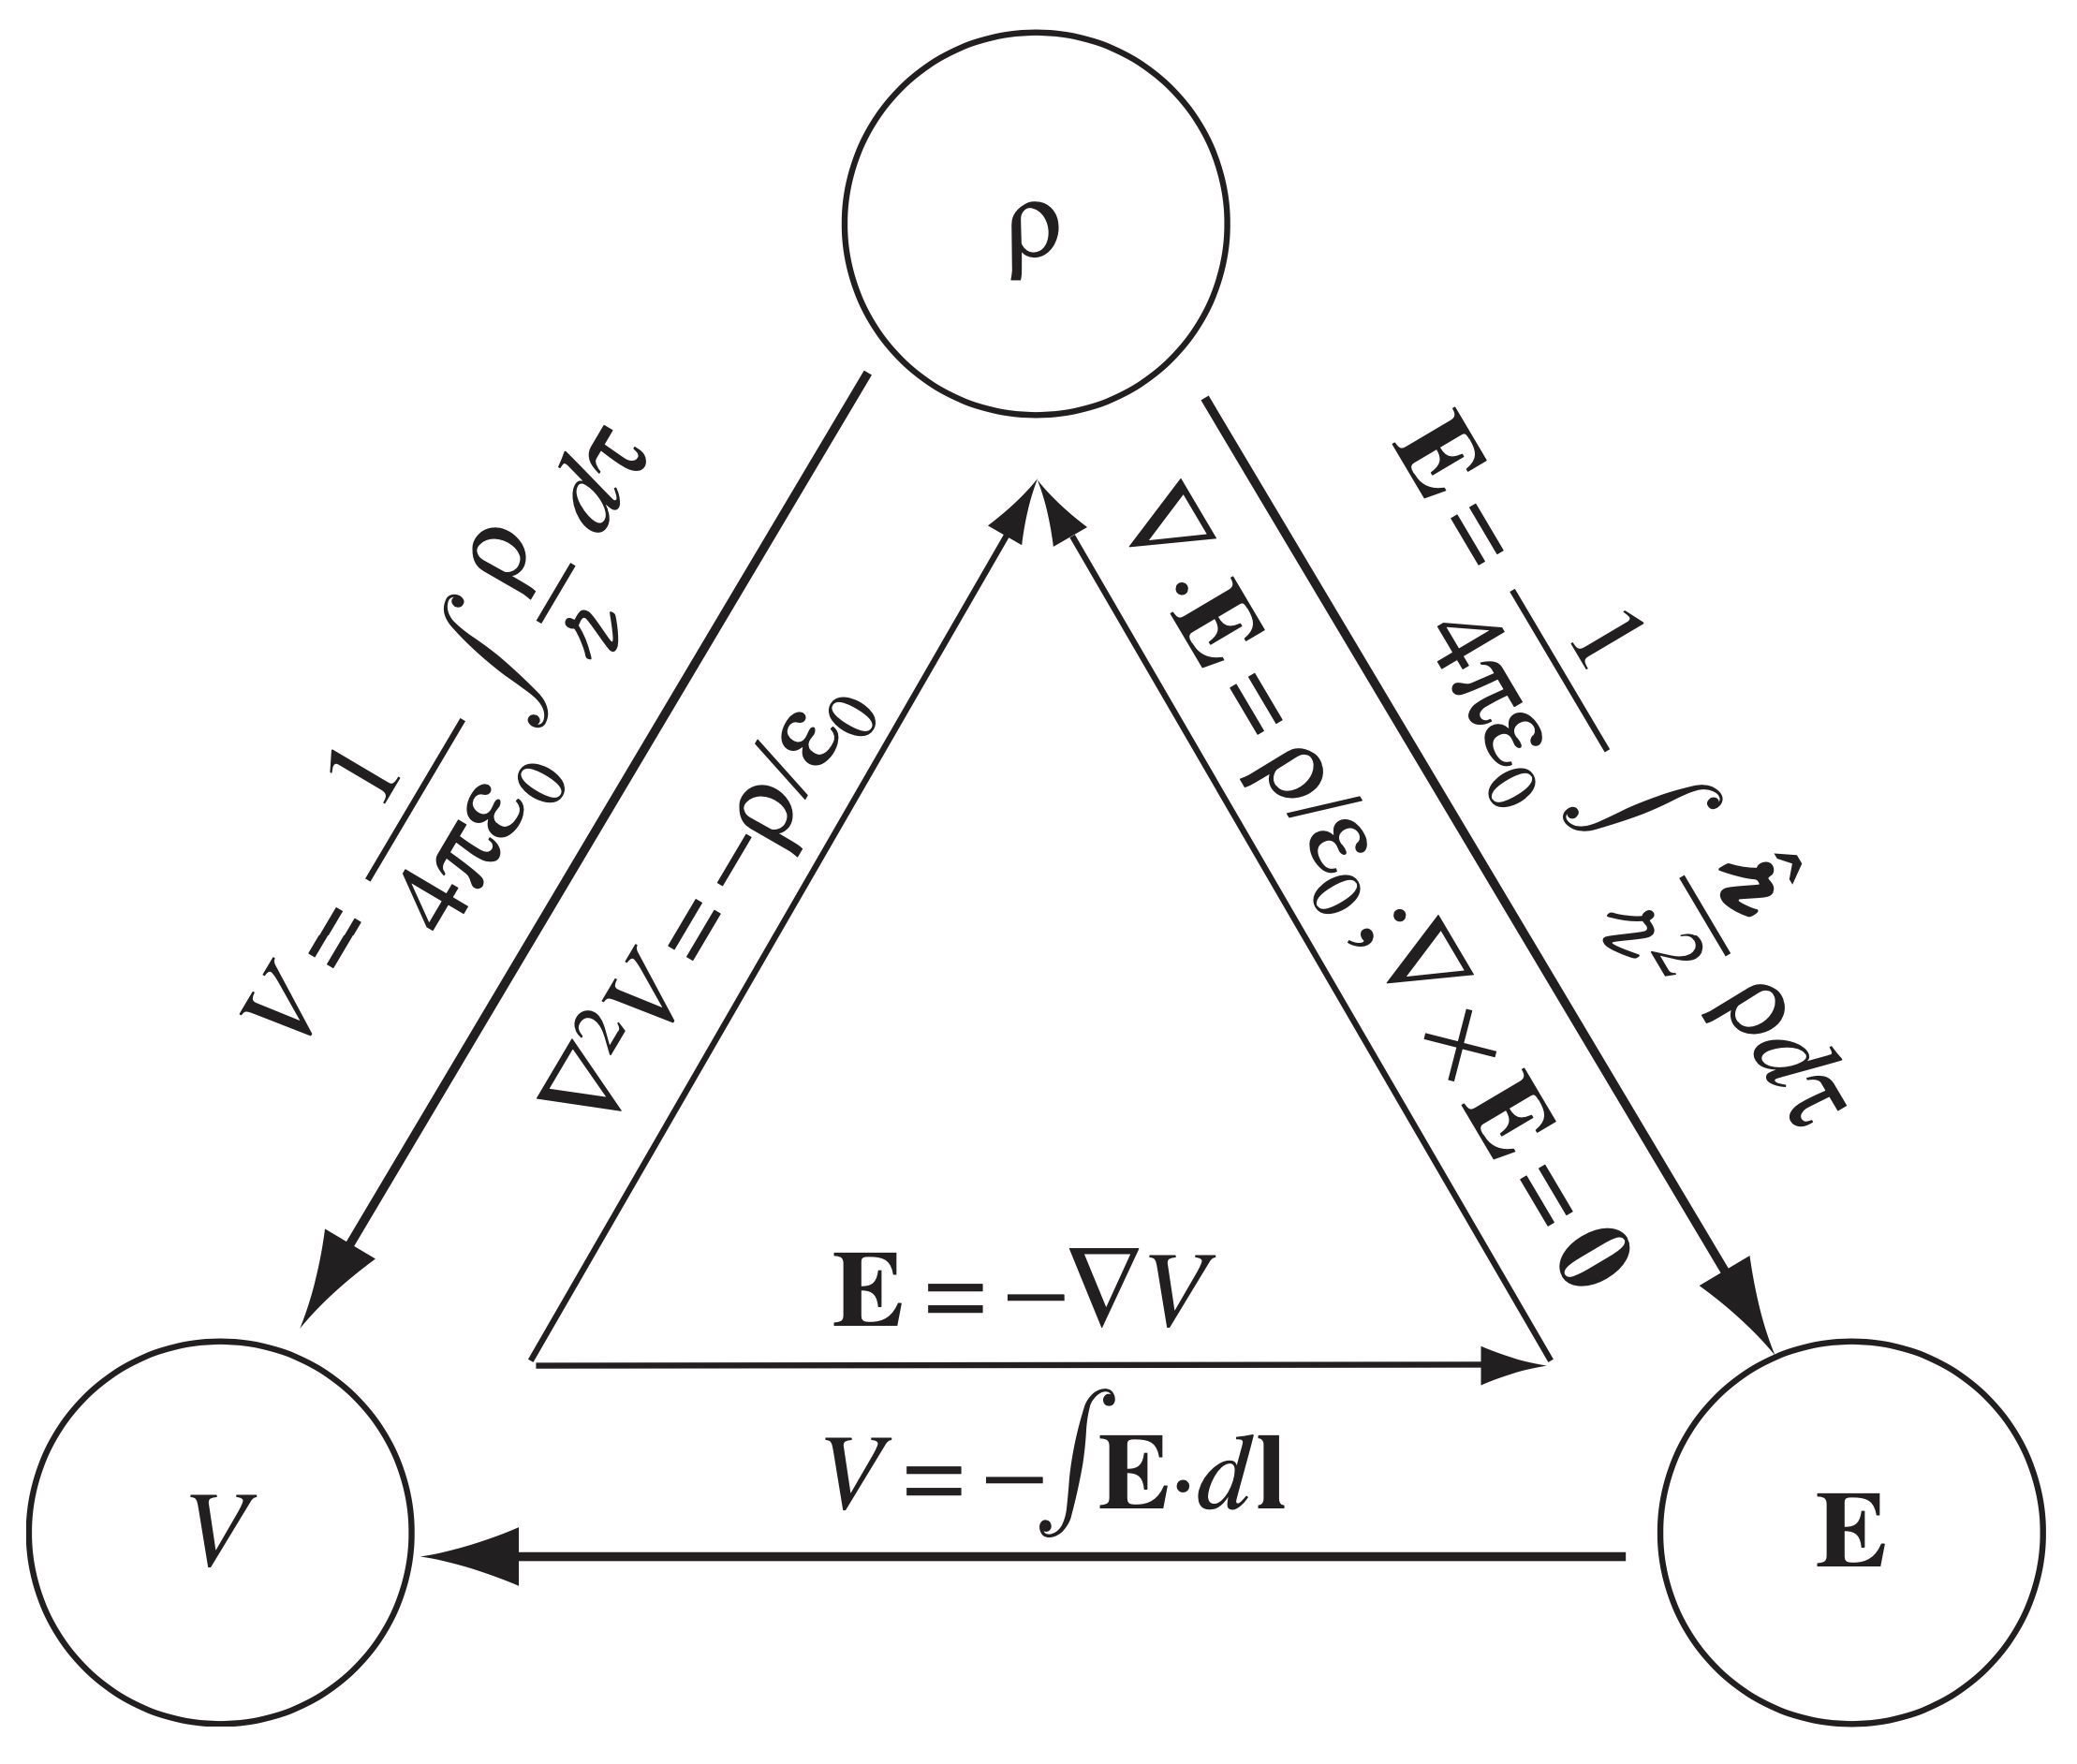
\includegraphics[scale=0.145]{em-triangle}
    \end{center}
}

\end{multicols*}

\end{document}